\chapter{Evaluation}

\newcommand{\cats}{\mathcal{C}}
\newcommand{\docs}{\mathcal{D}}
\newcommand{\train}{\mathcal{T}^r}
\newcommand{\test}{\mathcal{T}^e}


In order to evaluate the quality of the \aicat\ framework, several
aspects of the framework have been tested.  The three main areas
tested are quality of categorization, efficiency, and ease of use.
For testing the quality of categorization and efficiency, performance
is measured on categorization tasks using several different data sets.

Section \ref{Corpora} describes the data sets used during testing.
Section \ref{Quality} presents various measurements of how accurately
the framework performs on these data sets, and Section
\ref{Efficiency} discusses the computational efficiency of the
framework.  Section \ref{Applications} discusses the ease of use of
the framework in different contexts.


\section{Corpora}
\label{Corpora}

During development and testing, several data sets, or ``corpora,''
were used for framework testing and application building.  Since the
framework will behave differently on different data sets, it is
important to understand the characteristics of each corpus.  For
instance, different feature selection and categorization algorithms
may scale differently in relation to the size of the training corpus,
both in terms of efficiency and accuracy.\cite{chakrabarti:98} Also,
the specifics of the categorization problem in each corpus may be more
amenable to one categorization technique or another.

The main corpora used for evaluation are listed in this section.  Each
corpus consists of a set of documents $\docs$, a set of categories $\cats$ that
documents may be assigned to, and a domain-expert-made choice of
category assignments for each document.  These category assignments
are considered to be completely correct, and they form a standard
against which the TC system's categorization on the test documents can
be measured.  For each corpus, the set $\docs$ is divided into a
training set $\train$ and a test set $\test$.

Unless otherwise noted below, a list of common English words from
\cite{salton:89} was used as a ``stoplist,'' or a set of terms to
completely ignore when processing documents.  This is a common technique from
Information Retrieval,\cite{XXX-manning} as it is assumed that these words
possess little or no information about the target categories, and that
they will only slow processing and add noise to the data.


\subsection{ApteMod}


The ApteMod version of the Reuters-21578 corpus has become a
standard benchmark corpus in evaluating Text Categorization
systems.\cite{yang:99} It is a collection of 10,788 documents from the
Reuters financial newswire service, partitioned into a training set with 7769
documents and a test set with 3019 documents.  The total size of the
corpus is about 43 MB.  It is available for download from
\url{http://kdd.ics.uci.edu/databases/reuters21578/reuters21578.html}.

The distribution of categories in the ApteMod corpus is highly skewed,
with 36.7\% of the documents in the most common category, and only
0.0185\% (2 documents) in each of the five least common categories.
In fact, the original data source is even more skewed---in creating
the corpus, any categories that did not contain at least one document
in the training set and one document in the test set were removed from
the corpus.\cite{yang:99}

In the ApteMod corpus, each document belongs to one or more
categories.  There are 90 categories in the corpus.  The average
number of categories per document is 1.235, and the average number of
documents per category is about 148, or 1.37\% of the corpus.

Figure \ref{Corpora-catdist} shows the category distribution for all
four corpora discussed in this section.  The categories are plotted on
the horizontal axis, and the number of documents per category are
plotted on the vertical axis using a logarithmic scale.

\begin{figure}
\begin{center}
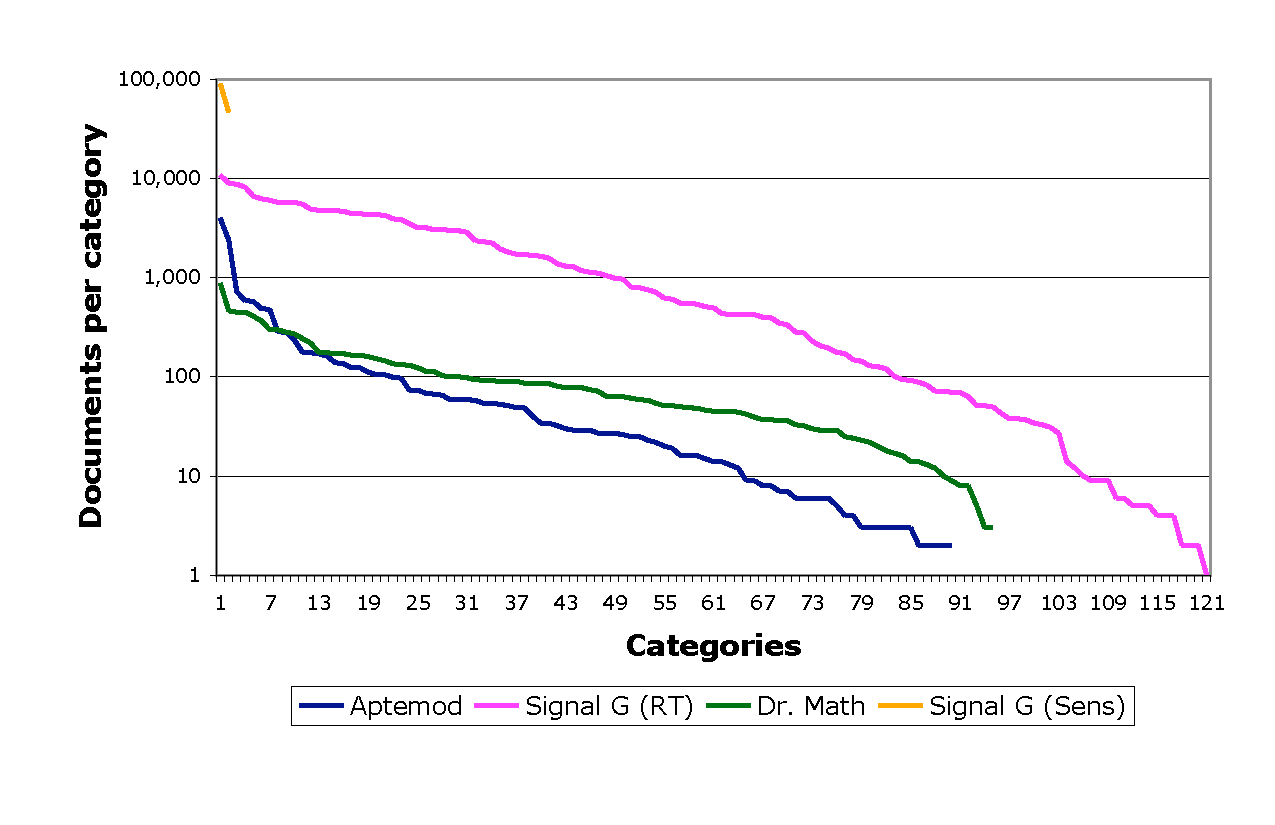
\includegraphics[width=\linewidth]{figures/Corpora-catdist.pdf}
\caption{Category distribution for the four test corpora}
\label{Corpora-catdist}
\end{center}
\end{figure}


\subsection{Dr. Math}

The Dr. Math corpus is a collection of 6,630 English-language messages
sent to the ``Ask Dr. Math'' question-and-answer service for
students.\cite{drmath} Each message has been manually assigned by a
domain expert to one or more categories,
with category names indicating both math topic and grade level,
e.g. ``High School Geometry.''  There are 95 categories in the
category set.  The ontology is generally not
separable into two separate category sets for independent topic and
level categorizations, in part because many topic and level
combinations like ``Elementary School Calculus'' don't exist in the
category scheme.

The 26 MB corpus is divided into a training set with 5,304 documents
and a test set with 1,326 documents.  As with the ApteMod corpus, the
category distribution is skewed, with 13.2\% of the documents in the
most common category and only 0.0452\% (3 documents) in the least
common category.  The average number of categories per document is
1.534, and the average number of documents per category is about 107,
or 1.61\% of the corpus.

The corpus is not available for direct download, but interested
parties may contact the author for details.


\subsection{Signal G (Sensitivity)}

The Signal G corpus consists of 136,630 financial announcement
documents from the Australian Stock Exchange (ASX)\cite{asx:02} issued
between January 4 and December 29, 2000.  Each documents has been
manually categorized by the ASX according to whether it indicates ``market
sensitivity'' or not.  Market sensitivity is a subjective label indicating
whether the given document has potential to affect the issuing
company's share value, trading volume, or other properties on the
exchange.  Every document is a member of either the ``sensitive'' or
``insensitive'' category---this can be viewed as two categories that
partition the corpus, or as a single category that some documents
belong to and others don't.  This discussion assumes the former.

The documents are divided into a training set of 95,525 documents and a
test set of 41,105 documents.  The total size of the corpus is about
342 MB.  Of the 136,630 corpus documents, about 34.0\% are marked as
market sensitive, and the rest are marked as insensitive.

\subsection{Signal G (Report Type)}

The same documents in the previous corpus can also be tagged with a
``report type'' category.  This category indicates the type of
business announcement contained in the document, and may take values
such as ``Notice of Annual General Meeting'' or ``Dividend Books
Closing.''  There are 121 categories in the corpus, with 7.91\%
(10,815 documents) belonging to the most common category, and ten
categories that contain five documents or fewer.  Thus the corpus
exhibits a high skew with respect to this category scheme, similar to
the ApteMod and Dr. Math corpora.

For this corpus with the Report Type labels, the same division between
training and test documents was used as with the Sensitivity labels.



\section{Quality of Categorization}
\label{Quality}

In order to evaluate the quality of the results generated by automatic
categorization systems, researchers usually evaluate the results of
the system on a controlled set of test documents.
\cite[pp. 9 \& 37]{sebastiani:02} This is the approach used here,
using the four corpora described in Section \ref{Corpora} as the test
sets.

It should be emphasized that this thesis does not claim to produce any
new results in the area of developing Text Categorization algorithms.
Descriptions of existing algorithms from the TC literature have formed
the basis for developing the \aicat\ framework.  The results presented
here should be considered successful if they align with results
already published in the literature---superior results should not be
expected.

\subsection{Performance Measures}
\label{measures}

Several statistical measures have become standard in the area of
evaluating Text Categorization systems.\cite[p. 33]{sebastiani:02}
Some of the most prevalant are based on the notions of
\emph{precision} and \emph{recall} from the field of Information
Retrieval.\cite{rijsbergen:79} Precision, often denoted by the symbol
$\pi$, measures the probability that a document assigned by the TC
system to a given category actually belongs to that category.
Conversely, recall, denoted by $\rho$, measures the probability that a
document actually belonging to a certain category will be assigned
during testing to that category.\cite[p. 33]{sebastiani:02}

The probabilities mentioned above can be estimated during testing by
comparing how often the TC system's category choices match the correct
categories.  A valuable tool for this analysis is the ``contingency
table,'' which summarizes the results of the experiment for a given
category.  Table \ref{onecat-contingency} shows a contingency table
for the category $c_i$, i.e. any arbitrary category in the
categorization scheme of the corpus.  Here, $A_i$, etc. represent the
number of documents that fall into the given situation, i.e. $A_i$ is
the number of test documents assigned to category $c_i$ by both the
expert and the TC system.

This allows us to estimate $\pi$ and $\rho$, whose true values are
$P(Expert=Y | System=Y)$ and $P(System=Y | Expert=Y)$, respectively,
in terms of the entries in the contingency table.  Since the number of
documents assigned to category $c_i$ by the TC system is $A_i+B_i$,
and the number assigned by the expert is $A_i+C_i$, our estimates for
$\pi$ and $\rho$ are $\frac{A_i}{A_i + B_i}$ and $\frac{A_i}{A_i +
C_i}$, respectively.



\begin{table}
\begin{center}
\begin{tabular}{|c|c|c|c|}
\cline{3-4}
\multicolumn{2}{c|}{} & \multicolumn{2}{c|}{\textbf{Expert choice}} \\
\cline{3-4}
\multicolumn{2}{c|}{} & Yes & No \\
\hline
\textbf{System} & Yes & $A_i$ & $B_i$ \\
\cline{2-4}
\textbf{choice} & No  & $C_i$ & $D_i$ \\
\hline
\end{tabular}
\end{center}
\caption{Contingency table for category $c_i$}
\label{onecat-contingency}
\end{table}


$\pi$ and $\rho$ give valuable information about the performance of a
TC system, but neither provides an isolated rating of the system's
quality.  The reason is that either measure can usually be improved in
a system to the detriment of the other.\cite[p. 35]{sebastiani:02} For
instance, the \emph{trivial acceptor} categorizer, which assigns every
document to every category, will have a perfect $\rho$ score of 1, but
its precision will be unacceptably low on any nontrivial task.

Therefore, a measure that combines $\pi$ and $\rho$ is desirable as an
overall measure of the quality of the TC system.  One such measure is
the $F_\beta$ measure, first introduced to the Information Retrieval
literature by van Rijsbergen \cite[ch. 7]{rijsbergen:79}.  It is
defined by the equation $F_\beta = \frac{(\beta^2 + 1)\pi\rho}{\beta^2
\pi + \rho}$, where $0 \leq \beta \leq \infty$.  The $\beta$ parameter
provides a continuous way to balance between the importance of $\pi$
and $\rho$, with values closer to 0 emphasizing $\pi$, values closer
to $\infty$ emphasizing $\rho$, and a value of 1 balancing the two
measures equally.  Without specific knowledge of an application's
requirements (for instance, whether false positives for a certain
category are more problematic than false negatives), one may presume
that $\pi$ and $\rho$ are equally important, and therefore the
literature often uses $F_1$ as a measure of the quality of a TC system
on a particular category.

${F_1}_i$ may be derived in terms of the entries of the per-category
contingency table as follows:

\begin{eqnarray*}
{F_1}_i 
 & = & \frac{ 2 \pi \rho}{\pi + \rho} \\
 & = & \frac{ \frac{2 {A_i}^2}{(A_i+B_i)(A_i+C_i)} } { \frac{A_i}{A_i+B_i} + \frac{A_i}{A_i+C_i} } \\
 & = & \frac{ 2 {A_i}^2 }                            { A_i(A_i+C_i) + A_i(A_i+B_i) } \\
 & = & \frac{ 2 A_i }                                { 2 A_i + B_i + C_i } \\
\end{eqnarray*}

Two other measures of categorization quality, \emph{error} and
\emph{accuracy}, are also sometimes encountered in the TC literature.
These are simple measures which can also be defined in terms of the
contingency table in Table \ref{onecat-contingency}: $error =
\frac{B_i+C_i}{A_i+B_i+C_i+D_i)}$, and $accuracy =
\frac{A_i+D_i}{A_i+B_i+C_i+D_i)}$.  In other words, error is the
proportion of the system's decisions that matched the expert's
choices, and accuracy is the proportion that did not.  As summarized
in \cite[p. 34]{sebastiani:02}, these are not always useful measures
of categorization quality, because the \emph{trivial rejector} (a
system that never assigns any documents to any category) will often
have a lower error and higher accuracy than most nontrivial
categorizers.  Nonetheless, error will be measured for the evaluation
tasks here, because it may give insight into the character of the
system's performance.


\subsection{Averaging Measures Across Categories}

Section \ref{measures} introduced several performance measures that
may be defined to evaluate a categorizer on a single category.  In
order to evaluate the categorizer's overall performance on the entire
set of test documents, it is desirable to combine the per-category
scores $\pi_i$, $\rho_i$, and ${F_1}_i$ into overall scores $\pi$,
$\rho$, and $F_1$ for the entire category set.

Two methods for doing this are standard in the literature.  The first
is called \emph{micro-averaging}, and sums the terms in the
contingency table for all categories simultaneously rather than in
per-category tables.  In other words, the micro-averaged $\pi$,
$\rho$, and $F_1$, notated $\pi^\mu$, $\rho^\mu$, and $F^\mu_1$, are
defined in terms of the per-category contingency tables by the
following equations.

\begin{displaymath}
 \pi^\mu = \frac{\sum_{i=1}^{|C|}{A_i}} {\sum_{i=1}^{|C|}{A_i+B_i}} \qquad
\rho^\mu = \frac{\sum_{i=1}^{|C|}{A_i}} {\sum_{i=1}^{|C|}{A_i+C_i}} \qquad
 F^\mu_1 = \frac{\sum_{i=1}^{|C|}{2 A_i}} {\sum_{i=1}^{|C|}{2 A_i+B_i+C_i}} \qquad
\end{displaymath}

Micro-averaging gives equal weight to each categorization decision
made by the system, or equivalently, to each document in the corpus,
regardless of the categories they belong to.

An alternative to micro-averaging is \emph{macro-averaging}, in which
the per-category scores $\pi_i$, $\rho_i$, and ${F_1}_i$ are simply
averaged to find the macro-averaged $\pi$, $\rho$, and $F_1$, notated
$\pi^M$, $\rho^M$, and $F^M_1$.  The following equations describe this
procedure.

\begin{displaymath}
 \pi^M = \frac{\sum_{i=1}^{|C|}{\pi_i}}   {|C|} \qquad
\rho^M = \frac{\sum_{i=1}^{|C|}{\rho_i}}  {|C|} \qquad
 F^M_1 = \frac{\sum_{i=1}^{|C|}{{F_1}_i}} {|C|} \qquad
\end{displaymath}

Macro-averaging gives equal weight to each category in the corpus,
regardless of how many documents they contain.  Thus it provides a
good counterpart to micro-averaging---macro-averaging will place more
emphasis on rare categories than micro-averaging, so reporting both
scores is typically useful to evaluate the system as a whole.

Note that the error and accuracy measures are unaffected by micro-
vs. macro-averaging, as shown in the following derivation.  This uses
the observation that $A_i+B_i+C_i+D_i = |\test|$, a consequence of the
fact that exactly one of the terms on the left side will be
incremented with each decision about whether a document from the test
set belongs to $c_i$ or not.

% XXX - really need to spread out this vertical spacing
% \begin{displaymath}
\begin{eqnarray*}
error^M
 & = & \frac{\sum_{i=1}^{|\cats|}{error_i}}  {|\cats|} \\
 & = & \frac{\sum_{i=1}^{|\cats|}{ \frac{B_i+C_i}{A_i+B_i+C_i+D_i} }} { \sum_{i=1}^{|\cats|}{1} } \\
 & = & \frac{\sum_{i=1}^{|\cats|}{ \frac{B_i+C_i}{|\test|} }}         { \sum_{i=1}^{|\cats|}{1} } \\
 & = & \frac{\sum_{i=1}^{|\cats|}{B_i+C_i}}                           { \sum_{i=1}^{|\cats|}{|\test|} } \\
 & = & \frac{\sum_{i=1}^{|\cats|}{B_i+C_i}}                           { \sum_{i=1}^{|\cats|}{A_i+B_i+C_i+D_i} } \\
 & = & error^\mu
\end{eqnarray*}
% \end{displaymath}

\begin{table}
\begin{center}
\begin{tabular}{|r c c c c c c c|}
\hline
method & $\rho^M$ & $\pi^M$ & $F_1^M$ & $\rho^\mu$ & $\pi^\mu$ & $F_1^\mu$ & error \\
\hline
NB       & .3659 & .4969 & .3959 & .7238 & .8514 & .7824 & .00555 \\
SVM      & .0836 & .2932 & .1148 & .4726 & .8657 & .6114 & .00807 \\
kNN      & \\
Baseline & .0135 & .0142 & .0137 & .1645 & .1664 & .1654 & .02287 \\
\hline
\end{tabular}
\end{center}
\caption{Results of \aicat\ on ApteMod corpus}
\end{table}

\begin{table}
\begin{center}
\begin{tabular}{|r c c c c c c c|}
\hline
method & $\rho^M$ & $\pi^M$ & $F_1^M$ & $\rho^\mu$ & $\pi^\mu$ & $F_1^\mu$ & error \\
\hline
NB  & ? & ? & .3886 & .7688 & .8245 & .7956 & .00544 \\
SVM & ? & ? & .5251 & .8120 & .9137 & .8599 & .00365 \\
kNN & ? & ? & .5242 & .8339 & .8807 & .8567 & .00385 \\
\hline
\end{tabular}
\end{center}
\caption{Results from \cite{yang:99} on ApteMod corpus}
\end{table}


\section{Efficiency}
\label{Efficiency}

\section{Applications}
\label{Applications}

\section{Dissemination}
XXX - perhaps eliminate this section

\subsection{Documentation}
\subsection{Community involvement}
